\section{Change of Axes}

\subsection{Change of Origin}
Consider the following diagrams:
\begin{mycenter}
	\tikzset{every picture/.style={line width=0.75pt}} %set default line width to 0.75pt        

	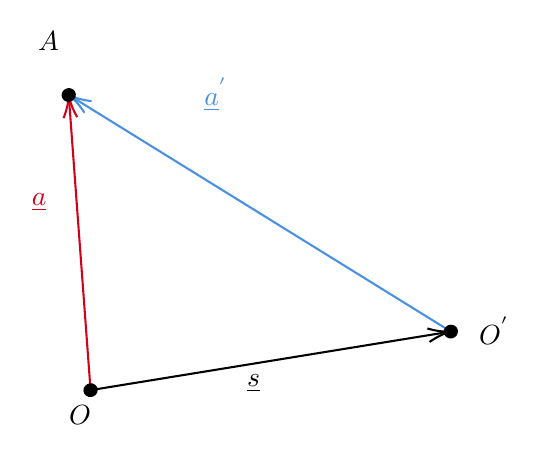
\begin{tikzpicture}[x=0.75pt,y=0.75pt,yscale=-1,xscale=1]
		%uncomment if require: \path (0,402); %set diagram left start at 0, and has height of 402

		%Straight Lines [id:da4437652617379132] 
		\draw [color={rgb, 255:red, 208; green, 2; blue, 27 }  ,draw opacity=1 ]   (163.8,233.14) -- (153.42,92.92) ;
		\draw [shift={(153.27,90.92)}, rotate = 85.76] [color={rgb, 255:red, 208; green, 2; blue, 27 }  ,draw opacity=1 ][line width=0.75]    (10.93,-3.29) .. controls (6.95,-1.4) and (3.31,-0.3) .. (0,0) .. controls (3.31,0.3) and (6.95,1.4) .. (10.93,3.29)   ;
		%Straight Lines [id:da6919359366246228] 
		\draw [color={rgb, 255:red, 74; green, 144; blue, 226 }  ,draw opacity=1 ]   (337.38,204.91) -- (154.97,91.97) ;
		\draw [shift={(153.27,90.92)}, rotate = 31.76] [color={rgb, 255:red, 74; green, 144; blue, 226 }  ,draw opacity=1 ][line width=0.75]    (10.93,-3.29) .. controls (6.95,-1.4) and (3.31,-0.3) .. (0,0) .. controls (3.31,0.3) and (6.95,1.4) .. (10.93,3.29)   ;
		%Shape: Ellipse [id:dp7599712014506931] 
		\draw  [fill={rgb, 255:red, 0; green, 0; blue, 0 }  ,fill opacity=1 ] (161.56,231.4) .. controls (160.52,232.62) and (160.68,234.39) .. (161.92,235.36) .. controls (163.16,236.32) and (165,236.11) .. (166.04,234.89) .. controls (167.08,233.67) and (166.92,231.89) .. (165.68,230.93) .. controls (164.45,229.97) and (162.6,230.18) .. (161.56,231.4) -- cycle ;
		%Straight Lines [id:da7071864815591788] 
		\draw    (163.8,233.14) -- (335.4,205.23) ;
		\draw [shift={(337.38,204.91)}, rotate = 170.76] [color={rgb, 255:red, 0; green, 0; blue, 0 }  ][line width=0.75]    (10.93,-3.29) .. controls (6.95,-1.4) and (3.31,-0.3) .. (0,0) .. controls (3.31,0.3) and (6.95,1.4) .. (10.93,3.29)   ;
		%Shape: Ellipse [id:dp6834980772983773] 
		\draw  [fill={rgb, 255:red, 0; green, 0; blue, 0 }  ,fill opacity=1 ] (335.14,203.17) .. controls (334.1,204.39) and (334.26,206.16) .. (335.5,207.12) .. controls (336.73,208.09) and (338.58,207.88) .. (339.62,206.66) .. controls (340.65,205.43) and (340.5,203.66) .. (339.26,202.7) .. controls (338.02,201.74) and (336.18,201.95) .. (335.14,203.17) -- cycle ;
		%Shape: Ellipse [id:dp029391721000904147] 
		\draw  [fill={rgb, 255:red, 0; green, 0; blue, 0 }  ,fill opacity=1 ] (151.03,89.18) .. controls (149.99,90.4) and (150.15,92.17) .. (151.39,93.13) .. controls (152.62,94.1) and (154.47,93.89) .. (155.51,92.67) .. controls (156.55,91.44) and (156.39,89.67) .. (155.15,88.71) .. controls (153.92,87.75) and (152.07,87.96) .. (151.03,89.18) -- cycle ;

		% Text Node
		\draw (217.09,81.19) node [anchor=north west][inner sep=0.75pt]  [color={rgb, 255:red, 74; green, 144; blue, 226 }  ,opacity=1 ] [align=left] {$\displaystyle \underline{a}^{'}$};
		% Text Node
		\draw (151.96,239.31) node [anchor=north west][inner sep=0.75pt]   [align=left] {$\displaystyle O$};
		% Text Node
		\draw (349.48,196.33) node [anchor=north west][inner sep=0.75pt]   [align=left] {$\displaystyle O^{'}$};
		% Text Node
		\draw (237.69,224.04) node [anchor=north west][inner sep=0.75pt]   [align=left] {$\displaystyle \underline{s}$};
		% Text Node
		\draw (137,59) node [anchor=north west][inner sep=0.75pt]   [align=left] {$\displaystyle A$};
		% Text Node
		\draw (134,137) node [anchor=north west][inner sep=0.75pt]  [color={rgb, 255:red, 208; green, 2; blue, 27 }  ,opacity=1 ] [align=left] {$\displaystyle \underline{a}$};
	\end{tikzpicture}
\end{mycenter}
Here we have 2 vectors
\begin{itemize}
	\item $\displaystyle \overrightarrow{OO}$
	\item $\displaystyle \overrightarrow{O^{'}O}$
\end{itemize}

\begin{tcolorbox}[title=Shift of Origin]
	The {\bf shift} of origin is represented by $\underline{s}$ is {\em relative} to $O$, then
	$$\underline{u} = \underline{a} = \underline{s} + \underline{a^{'}} \Rightarrow \underline{a^{'}} = \underline{a} - \underline{s}$$
\end{tcolorbox}
\begin{note}
	\underline{s} {\bf could depend on time}
\end{note}

\begin{note}
	Consider the following diagram

	\begin{mycenter}
		\tikzset{every picture/.style={line width=0.75pt}} %set default line width to 0.75pt        

		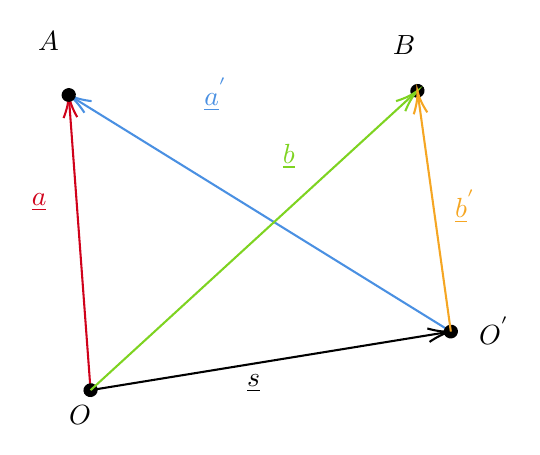
\begin{tikzpicture}[x=0.75pt,y=0.75pt,yscale=-1,xscale=1]
			%uncomment if require: \path (0,402); %set diagram left start at 0, and has height of 402

			%Straight Lines [id:da4437652617379132] 
			\draw [color={rgb, 255:red, 208; green, 2; blue, 27 }  ,draw opacity=1 ]   (163.8,233.14) -- (153.42,92.92) ;
			\draw [shift={(153.27,90.92)}, rotate = 85.76] [color={rgb, 255:red, 208; green, 2; blue, 27 }  ,draw opacity=1 ][line width=0.75]    (10.93,-3.29) .. controls (6.95,-1.4) and (3.31,-0.3) .. (0,0) .. controls (3.31,0.3) and (6.95,1.4) .. (10.93,3.29)   ;
			%Straight Lines [id:da6919359366246228] 
			\draw [color={rgb, 255:red, 74; green, 144; blue, 226 }  ,draw opacity=1 ]   (337.38,204.91) -- (154.97,91.97) ;
			\draw [shift={(153.27,90.92)}, rotate = 31.76] [color={rgb, 255:red, 74; green, 144; blue, 226 }  ,draw opacity=1 ][line width=0.75]    (10.93,-3.29) .. controls (6.95,-1.4) and (3.31,-0.3) .. (0,0) .. controls (3.31,0.3) and (6.95,1.4) .. (10.93,3.29)   ;
			%Shape: Ellipse [id:dp7599712014506931] 
			\draw  [fill={rgb, 255:red, 0; green, 0; blue, 0 }  ,fill opacity=1 ] (161.56,231.4) .. controls (160.52,232.62) and (160.68,234.39) .. (161.92,235.36) .. controls (163.16,236.32) and (165,236.11) .. (166.04,234.89) .. controls (167.08,233.67) and (166.92,231.89) .. (165.68,230.93) .. controls (164.45,229.97) and (162.6,230.18) .. (161.56,231.4) -- cycle ;
			%Straight Lines [id:da7071864815591788] 
			\draw    (163.8,233.14) -- (335.4,205.23) ;
			\draw [shift={(337.38,204.91)}, rotate = 170.76] [color={rgb, 255:red, 0; green, 0; blue, 0 }  ][line width=0.75]    (10.93,-3.29) .. controls (6.95,-1.4) and (3.31,-0.3) .. (0,0) .. controls (3.31,0.3) and (6.95,1.4) .. (10.93,3.29)   ;
			%Shape: Ellipse [id:dp6834980772983773] 
			\draw  [fill={rgb, 255:red, 0; green, 0; blue, 0 }  ,fill opacity=1 ] (335.14,203.17) .. controls (334.1,204.39) and (334.26,206.16) .. (335.5,207.12) .. controls (336.73,208.09) and (338.58,207.88) .. (339.62,206.66) .. controls (340.65,205.43) and (340.5,203.66) .. (339.26,202.7) .. controls (338.02,201.74) and (336.18,201.95) .. (335.14,203.17) -- cycle ;
			%Shape: Ellipse [id:dp029391721000904147] 
			\draw  [fill={rgb, 255:red, 0; green, 0; blue, 0 }  ,fill opacity=1 ] (151.03,89.18) .. controls (149.99,90.4) and (150.15,92.17) .. (151.39,93.13) .. controls (152.62,94.1) and (154.47,93.89) .. (155.51,92.67) .. controls (156.55,91.44) and (156.39,89.67) .. (155.15,88.71) .. controls (153.92,87.75) and (152.07,87.96) .. (151.03,89.18) -- cycle ;
			%Shape: Ellipse [id:dp487875436345539] 
			\draw  [fill={rgb, 255:red, 0; green, 0; blue, 0 }  ,fill opacity=1 ] (319.03,87.18) .. controls (317.99,88.4) and (318.15,90.17) .. (319.39,91.13) .. controls (320.62,92.1) and (322.47,91.89) .. (323.51,90.67) .. controls (324.55,89.44) and (324.39,87.67) .. (323.15,86.71) .. controls (321.92,85.75) and (320.07,85.96) .. (319.03,87.18) -- cycle ;
			%Straight Lines [id:da2129903038772052] 
			\draw [color={rgb, 255:red, 126; green, 211; blue, 33 }  ,draw opacity=1 ]   (163.8,233.14) -- (319.79,90.27) ;
			\draw [shift={(321.27,88.92)}, rotate = 137.51] [color={rgb, 255:red, 126; green, 211; blue, 33 }  ,draw opacity=1 ][line width=0.75]    (10.93,-3.29) .. controls (6.95,-1.4) and (3.31,-0.3) .. (0,0) .. controls (3.31,0.3) and (6.95,1.4) .. (10.93,3.29)   ;
			%Straight Lines [id:da6831431930714746] 
			\draw [color={rgb, 255:red, 245; green, 166; blue, 35 }  ,draw opacity=1 ]   (337.38,204.91) -- (321.54,90.9) ;
			\draw [shift={(321.27,88.92)}, rotate = 82.09] [color={rgb, 255:red, 245; green, 166; blue, 35 }  ,draw opacity=1 ][line width=0.75]    (10.93,-3.29) .. controls (6.95,-1.4) and (3.31,-0.3) .. (0,0) .. controls (3.31,0.3) and (6.95,1.4) .. (10.93,3.29)   ;

			% Text Node
			\draw (217.09,81.19) node [anchor=north west][inner sep=0.75pt]  [color={rgb, 255:red, 74; green, 144; blue, 226 }  ,opacity=1 ] [align=left] {$\displaystyle \underline{a}^{'}$};
			% Text Node
			\draw (151.96,239.31) node [anchor=north west][inner sep=0.75pt]   [align=left] {$\displaystyle O$};
			% Text Node
			\draw (349.48,196.33) node [anchor=north west][inner sep=0.75pt]   [align=left] {$\displaystyle O^{'}$};
			% Text Node
			\draw (237.69,224.04) node [anchor=north west][inner sep=0.75pt]   [align=left] {$\displaystyle \underline{s}$};
			% Text Node
			\draw (137,59) node [anchor=north west][inner sep=0.75pt]   [align=left] {$\displaystyle A$};
			% Text Node
			\draw (308,61) node [anchor=north west][inner sep=0.75pt]   [align=left] {$\displaystyle B$};
			% Text Node
			\draw (134,137) node [anchor=north west][inner sep=0.75pt]  [color={rgb, 255:red, 208; green, 2; blue, 27 }  ,opacity=1 ] [align=left] {$\displaystyle \underline{a}$};
			% Text Node
			\draw (255,113) node [anchor=north west][inner sep=0.75pt]  [color={rgb, 255:red, 126; green, 211; blue, 33 }  ,opacity=1 ] [align=left] {$\displaystyle \underline{b}$};
			% Text Node
			\draw (338,135) node [anchor=north west][inner sep=0.75pt]  [color={rgb, 255:red, 245; green, 166; blue, 35 }  ,opacity=1 ] [align=left] {$\displaystyle \underline{b}^{'}$};

		\end{tikzpicture}
	\end{mycenter}
	Let $\underline{a}$ and $\underline{b}$ represent  vectors  to $A$ and $B$ relative to $O$. Similarly let $\underline{a^{'}}$ and $\underline{b^{'}}$ represent vectors relative to $O^{\ '}$ .  Then:

	$$\underline{a}^{'}  \ - \ \underline{b}^{'}  = (\underline{a} - \underline{s})\  - \ (\underline{b}-\underline{s})  = \underline{a} - \underline{b}$$

	As we can see the {\bf displacement} from $\underline{a}$  to $\underline{b}$ is the {\bf same} as the {\bf displacement} from $\underline{a}^{'}$ to $\underline{b}^{'}$.
\end{note}


\subsection{Shifting and Changing Unit Vectors}

